\subsection{System Architecture}
To help \mbox{D-FLAT} profit from machine learning techniques an architecture based on the one proposed in ~\cite{claspfolio} was used. It is shown in Figure~\ref{impl:sysarch}. First instance features are extracted, then a prediction which solver configuration will be the best is made using machine learning algorithms and finally \mbox{D-FLAT} is launched with the predicted configuration.
A Python script was implemented to handle the control flow such that the user only has to supply the instance and learning database. Furthermore some modifications to \mbox{D-FLAT} were made to allow the configuration of the solver.

\begin{figure}[h]
	\center
	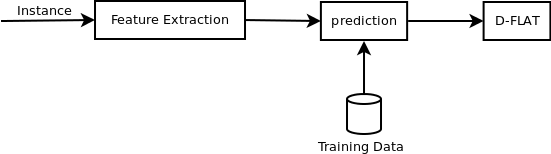
\includegraphics[scale=0.6]{figures/sysarch.png}
	\caption{System Architecture of \mbox{D-FLAT} with Learning\label{impl:sysarch}}
\end{figure}

\subsection{Modifications to \mbox{D-FLAT}}
To the default configuration four different \inline$clasp$ configurations were added using the class \inline$clasp_fascade$ of its library. The three configurations \inline$jumpy$, \inline$frumpy$ and \inline$crafty$ aim to copy the portfolios provided by \inline$clasp$, while \inline$nopre$ instructs \inline$clasp$ to skip any ASP preprocessing and start solving directly. These configurations were added to the \inline$solver::Asp$ class in \mbox{D-FLAT}. Users can set the desired portfolio by using the \inline$--portfolio$ flag followed by the name of the portfolio in the command line arguments.

\subsection{Feature Extraction}
Another new flag \inline$--ext-feat$ instructs \mbox{D-FLAT} to stop processing after decomposing the instance and print out its features in machine readable format. This is used for feature extraction. Additional feature extractors can be implemented by writing subclasses of \inline$FeatureExtractor$ and adding corresponding instances to the list \inline$felist$ in the \inline$Algorithm$ class.

Apart from features extractable from \mbox{D-FLAT}, also features from other sources are used. Features of the encoding are extracted using \inline$gringo$s~\cite{Gringo} \inline$--gstats$ flag and some features are extracted directly from the instance file. Also some features of the tree decomposition specified by the user are used. A complete list of available features can be seen in Table~\ref{tbl:feat}. New features from other sources can be added by creating subclasses of \inline$FeatureExtractor$ in the Python script  \inline$Learner$.

\begin{table}[h]
	\center
	\begin{tabular}{|l|l|l|}
		\hline
		Name & Description & Origin \\
		\hline
		\inline$gcomponents$ & number of components & \inline$gringo$\\
		\inline$gnontrivial$ & number of nontrivial components & \inline$gringo$\\
		\inline$gpredicates$ & number of predicates & \inline$gringo$ \\
		\inline$gconstraints$ & number of constraints & \inline$gringo$\\
		\inline$nbredgefacts$ & number of edge facts & instance file\\
		\inline$nbredgepred$ & number of edge predicates & user \\
		\inline$defjoin$ & $1$ if \mbox{D-FLAT}s default join was used, $0$ otherwise & user\\
		\inline$normalization$ & the normalization used (non-, semi-, weak-normalized) & user\\
		\inline$heuristic$ & the heuristic used to create the tree decomposition & user\\
		\inline$dw$ & the decomposition width of the tree decomposition & \mbox{D-FLAT}\\
		\hline
	\end{tabular}
	\caption{Features of the datasets}
	\label{tbl:feat}
\end{table}

\subsection{Learner}
The program \inline$Learner$ has been developed to handle all machine learning related tasks. \inline$Learner$ supports $3$ subcommands \inline$learn, genmod$ and \inline$solve$. 
\inline$learn$ instructs \inline$Learner$ to build the learning base, or training set as it is often called and save it in \inline$csv$ style. 
\inline$genmod$ generates a Support Vector Machine model based on the training set and \inline$solve$ is used to actually solve instances. %Detailed information on the different subtools is given in the following paragraphs.

Basic configuration of \inline$Learner$ is done with the \inline$config.xml$ file in its main directory. Here instances to build the learning base and paths to the required executables for the feature extraction need to be specified. For further detail on the configuration look at the example provided in the distribution. Table~\ref{tbl:req} shows \inline$Learner$'s system requirements.

\begin{table}[h]
	\center
	\begin{tabular}{ll}
		Requirement & Version\\
		Python & $\geq2.7$\\
		Gringo & $\geq3.0$\\
		scikit-learn & $\geq0.10$\\
		D-FLAT learn & $\geq0.01$
	\end{tabular}
	\caption{Learner system requirements \label{tbl:req}}
\end{table}

\paragraph{\inline$learn$}
It is encouraged to use \inline$learn$ to build training sets. For every instance provided in the \inline$config.xml$ \inline$Learner$ first extracts the features of the instance using subclasses of \inline$FeatureExtractor$ to obtain them. Then it calls \mbox{D-FLAT} with each portfolio and measures the runtime using GNU time~\cite{www:time}.
Using the flags \inline$--mtime$ and \inline$--reslimit$ the execution time and resource usage can be limited for each process. If one of these limits is reached, \inline$Learner$ kills the instance and reports $-100$ as runtime, telling that this instance was not solvable with the respective portfolio. It then writes all features and runtimes to a file. The destination of this file can be specified using \inline$--learningbase$. As default \inline$learningbase.csv$ is used. The learning base can be used to build the machine learning model using \inline$genmod$.

\paragraph{\inline$genmod$}
Invoking this command tells \inline$Learner$ to build a model of the learning base specified by the flag \inline$--learningbase$. Support Vector Machines as implemented by scikit-learn~\cite{www:scikit} are used as classifier. Numerical features are scaled such that they have $0$ mean and unit variance using scikit-learns \inline$StandardScaler$. 
Nominal features are encoded using \inline$1-of-K$ encoding, i.e. for $K$ different values each value is represented by a binary vector of $K$ length where exactly $1$ bit has the value $1$ and all others $0$.
After preprocessing the model is fitted to the learning base and saved to \inline$default.mod$. To choose a different location \inline$--model$ can be used.

\paragraph{\inline$solve$}
is used to solve instances with the best portfolio predicted by the model generated by \inline$genmod$. The model is specified using \inline$--model$, \inline$-e$ is used to specify the edge predicates, other arguments for \mbox{D-FLAT} can be specified as string using \inline$--arg$.
Learner then predicts the best portfolio based on the specified model and launches \mbox{D-FLAT} with it. Any output generated by \mbox{D-FLAT} is shown in the terminal.



